\documentclass[12pt,twoside]{article}
%\date{}   %uncommenting this erases the date
\usepackage{graphicx}
\usepackage{amsmath}
\usepackage{amssymb}
%\usepackage{natbib}
%\usepackage{verbatim}
\usepackage{floatpag}
\usepackage{subeqnarray}
\usepackage{mathrsfs}    %for special characters
\usepackage{cancel}  % to set terms in an equation to zero



\setlength{\textheight}     {9.0in}
\setlength{\textwidth}      {6.5in}
\setlength{\oddsidemargin}  {0.0in}
\setlength{\evensidemargin} {0.0in}
\setlength{\topmargin}      {0.0in}
\setlength{\headheight}     {0.0in}
\setlength{\headsep}        {0.0in}
\setlength{\hoffset}        {0.0in}
\setlength{\voffset}        {0.0in}
\setlength{\parindent}      {0.0in}      %starting new line at extreme left

\graphicspath{{Figures/}}

\newcommand{\astrut}{\usebox{\astrutbox}}

\newcommand\GaPQ{\ensuremath{G_a(P,Q)}}
\newcommand\GsPQ{\ensuremath{G_s(P,Q)}}
\newcommand\p{\ensuremath{\partial}}
\newcommand\tti{\ensuremath{\rightarrow\infty}}
\newcommand\kgd{\ensuremath{k\gamma d}}
\newcommand\shalf{\ensuremath{{\scriptstyle\frac{1}{2}}}}
\newcommand\sh{\ensuremath{^{\shalf}}}
\newcommand\smh{\ensuremath{^{-\shalf}}}
\newcommand\squart{\ensuremath{{\textstyle\frac{1}{4}}}}
\newcommand\thalf{\ensuremath{{\textstyle\frac{1}{2}}}}
\newcommand\Gat{\ensuremath{\widetilde{G_a}}}
\newcommand\ttz{\ensuremath{\rightarrow 0}}
\newcommand\ndq{\ensuremath{\frac{\mbox{$\partial$}}{\mbox{$\partial$} n_q}}}
\newcommand\sumjm{\ensuremath{\sum_{j=1}^{M}}}
\newcommand\pvi{\ensuremath{\int_0^{\infty}%
  \mskip \ifCUPmtlplainloaded -30mu\else -33mu\fi -\quad}}

\newcommand\etal{\mbox{\textit{et al.}}}
\newcommand\etc{etc.\ }
\newcommand\eg{e.g.\ }



\newcommand{\bs}  [1]{\boldsymbol{#1}}
\newcommand{\del} {\nabla}
\newcommand{\bsh}  [1]{\boldsymbol{\hat{#1}}}
\newcommand{\ul}  {\underline}
\newcommand{\ol}  {\overline}
\newcommand{\pp} [2]{\frac{\p{#1}}{\p{#2}}}
\newcommand{\dd} [2]{\frac{d{#1}}{d{#2}}}
\newcommand{\lam}  [1]{{#1}^{\tiny{\lambda}}}
\newcommand{\conj} [1]{{#1}^*}
\newcommand{\mods} [1]{ \vert {#1} \vert ^2}


\begin{document}

\title{Singularity formation in Birkhoff-Rott equation}


\author{Raghav Singhal}

\maketitle
\section{Algorithm}
In this work we introduce a new integration scheme to resolve singularity formation in the Birkhoff-Rott equation. We desingularize the birkhoff-rott equation for a periodic vortex sheet by doing a line integral around the singulart part of the kernel. The line integral is done on a rectangular region where the height is the thickness, $b_j$, and the width is $\alpha*2b_j$ where $\alpha$ is a free parameter in the model. 

\section{Discretization}
The integration scheme is defined as :
\begin{equation}
\frac{dx_j}{dt}=\frac{-1}{2N} \sum_{x_k \in \Omega /S} \frac{\sinh(2\pi(y_j - y_k))}{\cosh(2\pi(x_j - x_k)) - \cos(2\pi(y_j - y_k)) + \delta^2}
\end{equation}

\begin{equation}
\frac{dy_j}{dt}=\frac{1}{2N} \sum_{x_k \in \Omega /S_j} \frac{\sin(2\pi(x_j - x_k))}{\cosh(2\pi(x_j - x_k)) - \cos(2\pi(y_j - y_k)) + \delta^2}
\end{equation}

where $\Omega$ is the curve  and $S_j$ is the singular part of the integral with width $\alpha*2b_j$. Then we compute the line integral around $\partial S_j$ , which in our model is a rectangular filament with the inner and outer curves as its boundary.

\begin{equation}
d\bs x=\sum_{x_k \in \partial S_j}(\Delta u_{jk})(\cos\theta_k\bs e_x + \sin\theta_k \bs e_y)
\end{equation}
where $\Delta u=\frac{1}{2\pi}h_k(log(r_j)$ and 
\begin{equation}
h_k=distance(x_k,x_{k+1})
\end{equation}

\begin{equation}
r_k=distance(x_j,x_k)
\end{equation}

\begin{equation}
\tan\theta_k=\frac{y_{k+1} - y_k}{x_{k+1} -x_k}
\end{equation}

We used the standard runge-Kutta fourth order scheme with a point removal scheme.

\section{Observations}
1. We observed that around the central region of the curve an elliptical region develops         as shown in the figures below. \\

2. Points tend to get closer towards the central region and without a point insertion and point removal scheme we cannot proceed further in time to obtain regular motion.\\

3. The central region is very sensitive to the $\alpha$ value we choose as the thickness reduces at the end of the ellptical region.

\begin{figure}[ht]
\centering
\begin{minipage}[b]{0.45\linewidth}
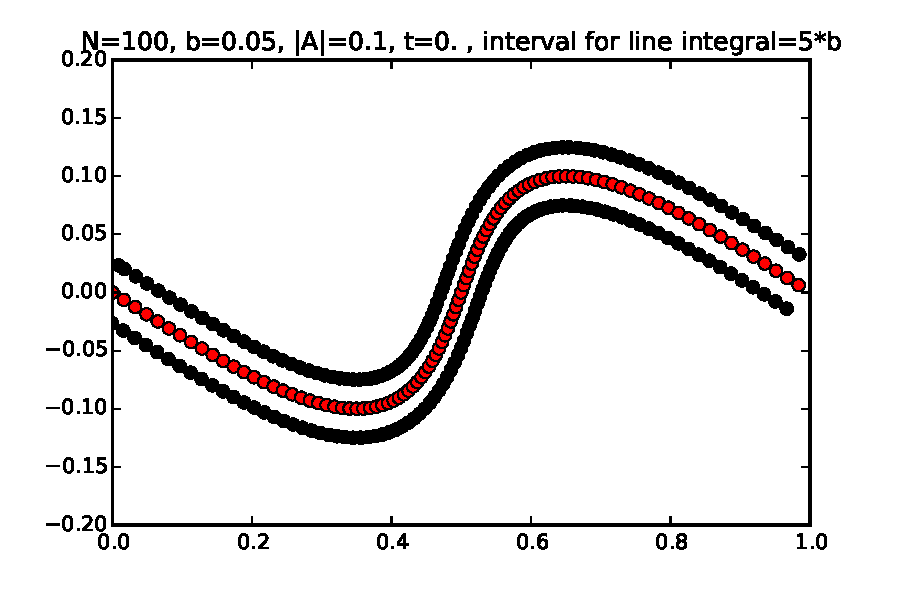
\includegraphics[width=3in,height=2in]{t00.pdf}
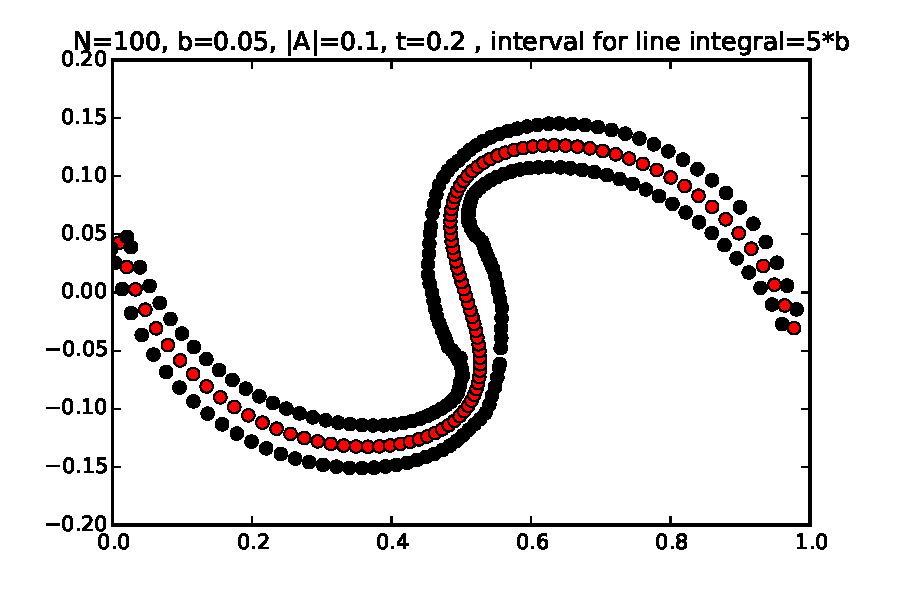
\includegraphics[width=3in,height=2in]{t02.pdf}
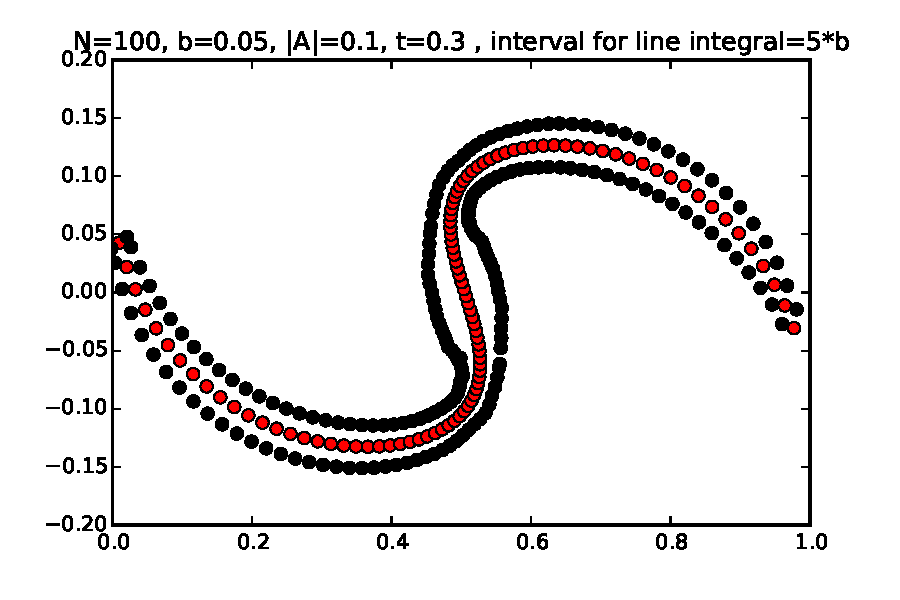
\includegraphics[width=3in,height=2in]{t03.pdf}
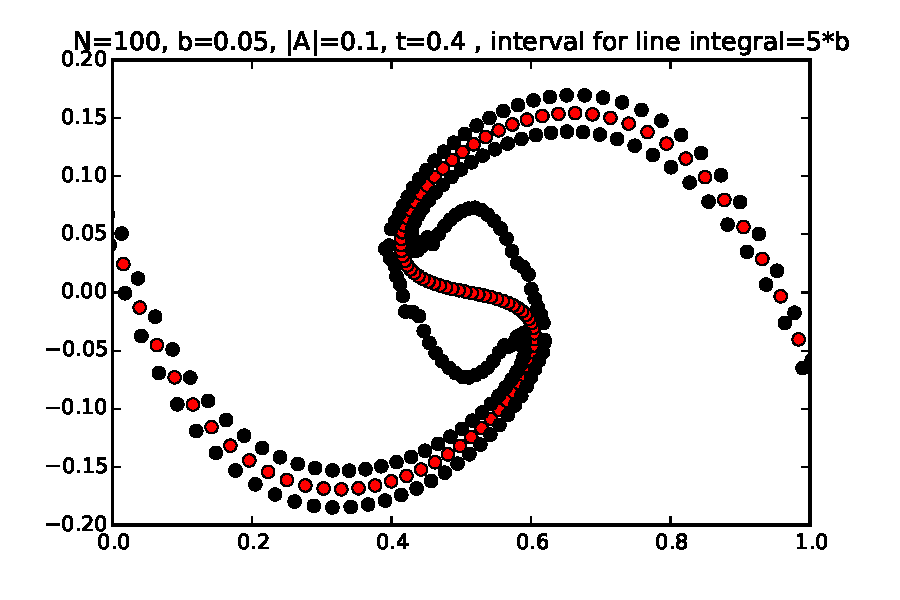
\includegraphics[width=3in,height=2in]{t04.pdf}
\caption{$N=500 , \delta=0.05 ,  t=0.45$ }
\end{minipage}
\quad
\begin{minipage}[b]{0.45\linewidth}
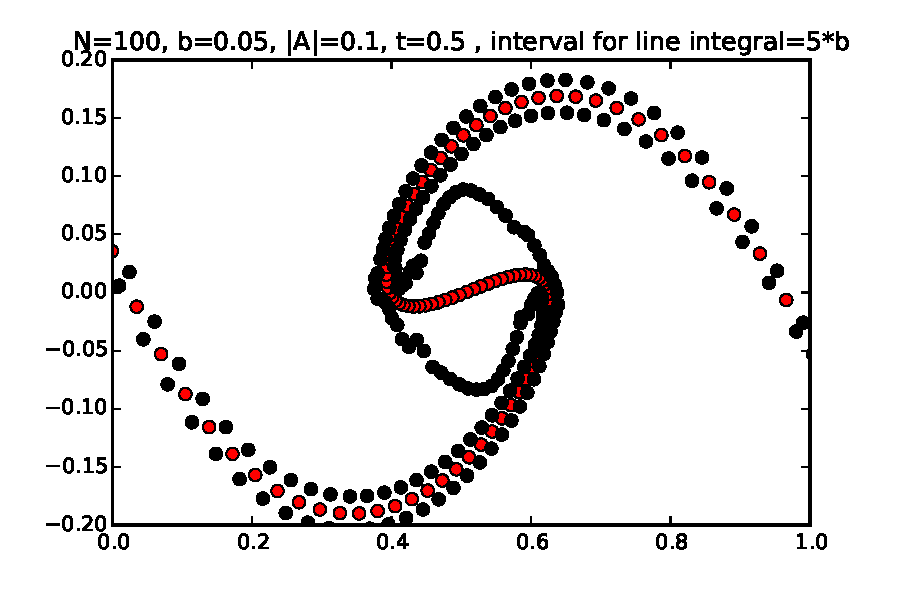
\includegraphics[width=3in,height=2in]{t05.pdf}
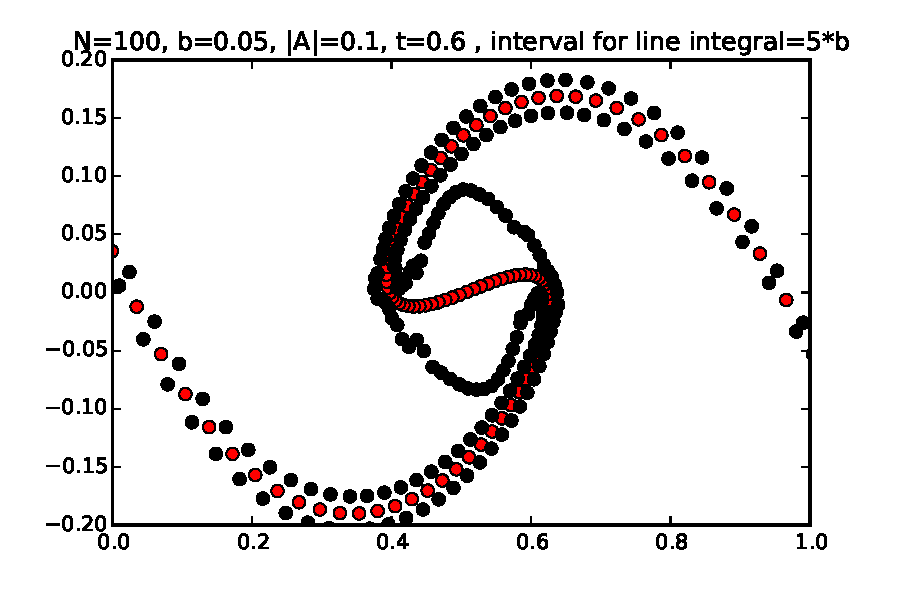
\includegraphics[width=3in,height=2in]{t06.pdf}
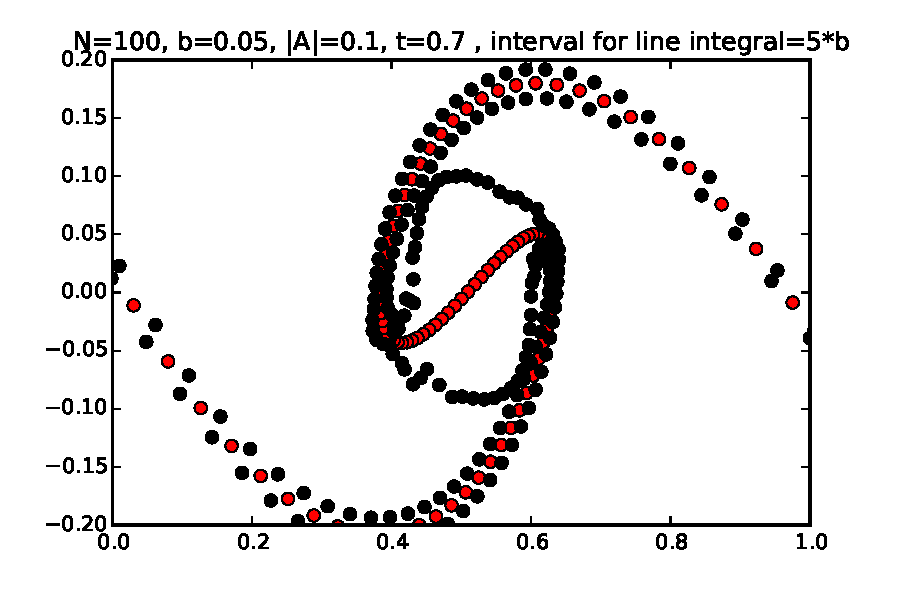
\includegraphics[width=3in,height=2in]{t07.pdf}
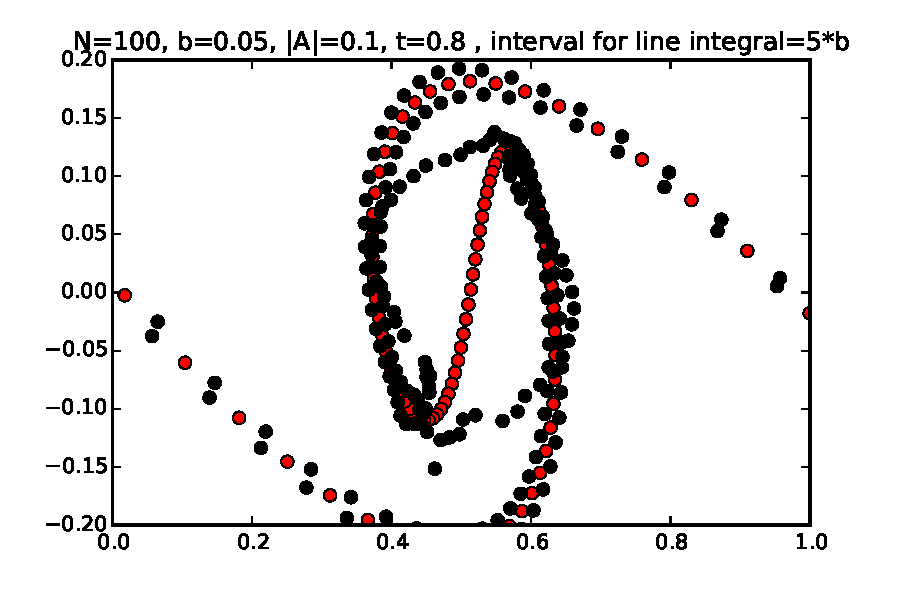
\includegraphics[width=3in,height=2in]{t08.pdf}
\caption{$N=500 , \delta=0.05 ,  t=0.52$ }
\end{minipage}
\end{figure}

\begin{figure}[ht]
\centering
\begin{minipage}[b]{0.45\linewidth}
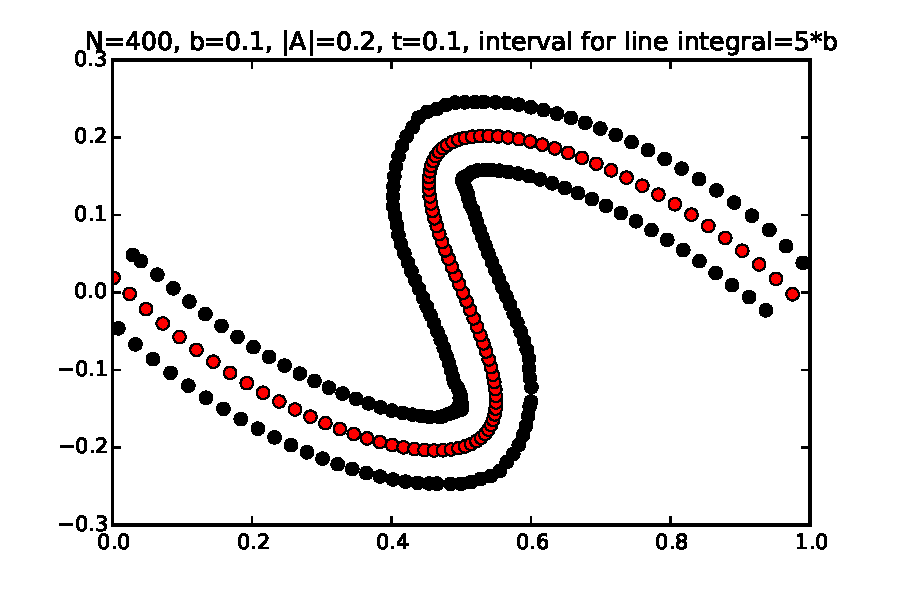
\includegraphics[width=3in,height=2in]{t01_B01.pdf}
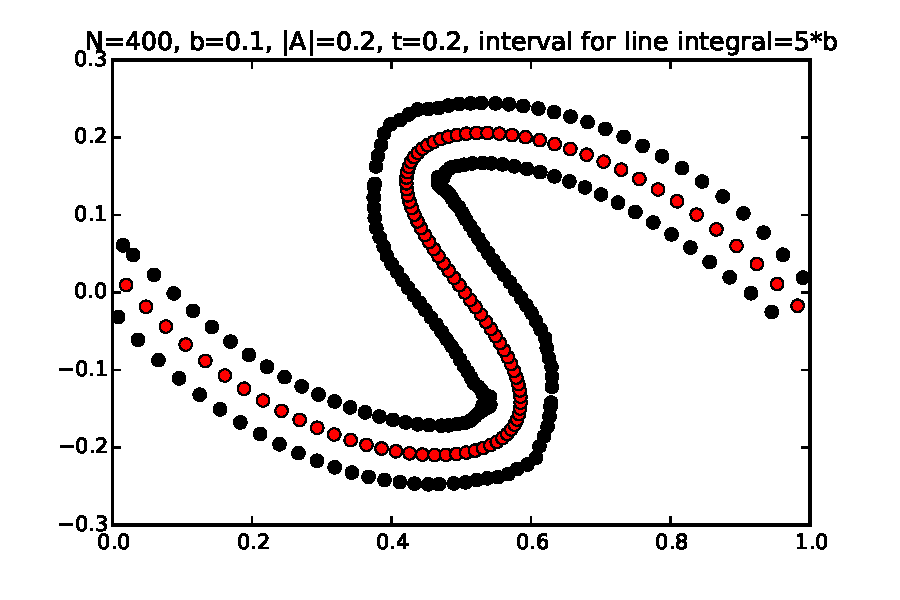
\includegraphics[width=3in,height=2in]{t02_B01.pdf}
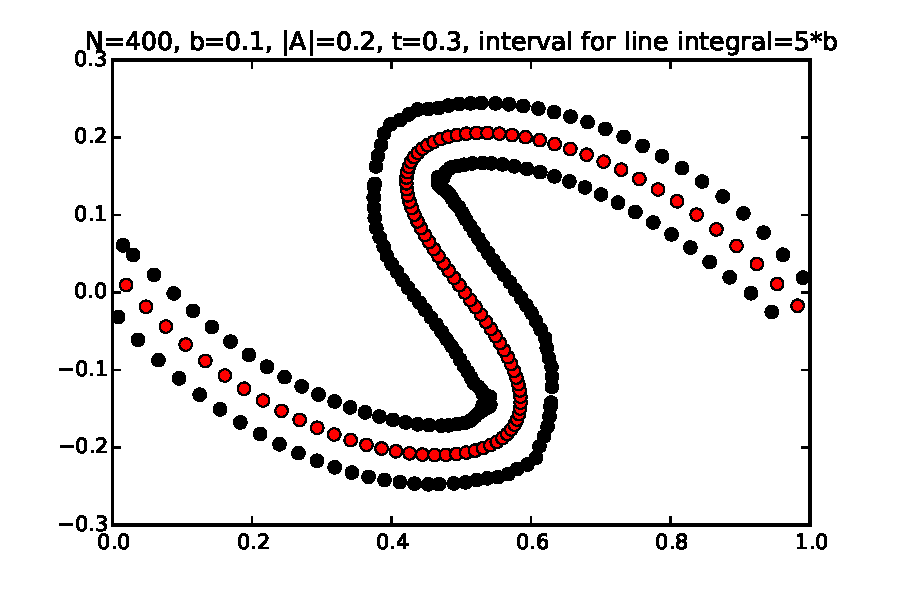
\includegraphics[width=3in,height=2in]{t03_B01.pdf}
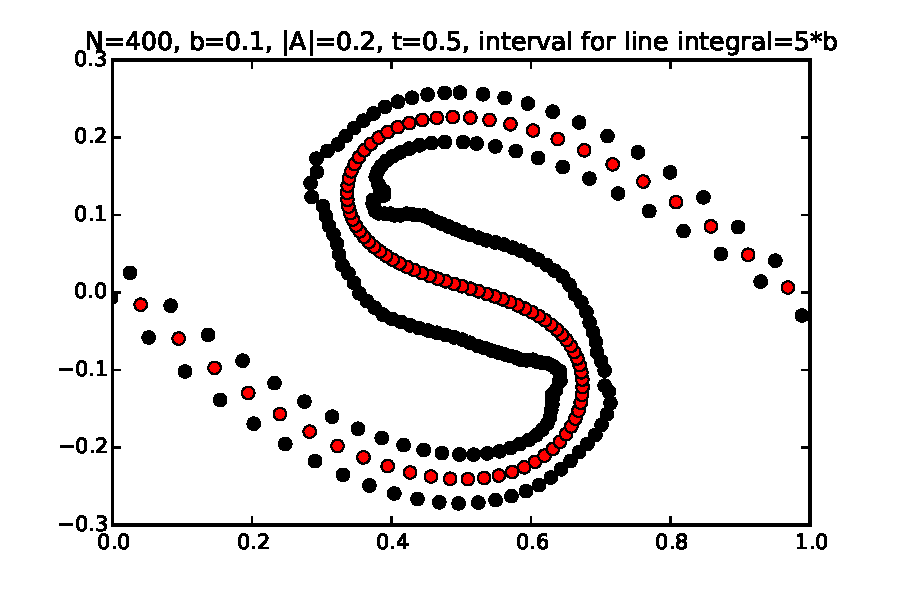
\includegraphics[width=3in,height=2in]{t05_B01.pdf}
\caption{$N=500 , \delta=0.05 ,  t=0.45$ }
\end{minipage}
\quad
\begin{minipage}[b]{0.45\linewidth}
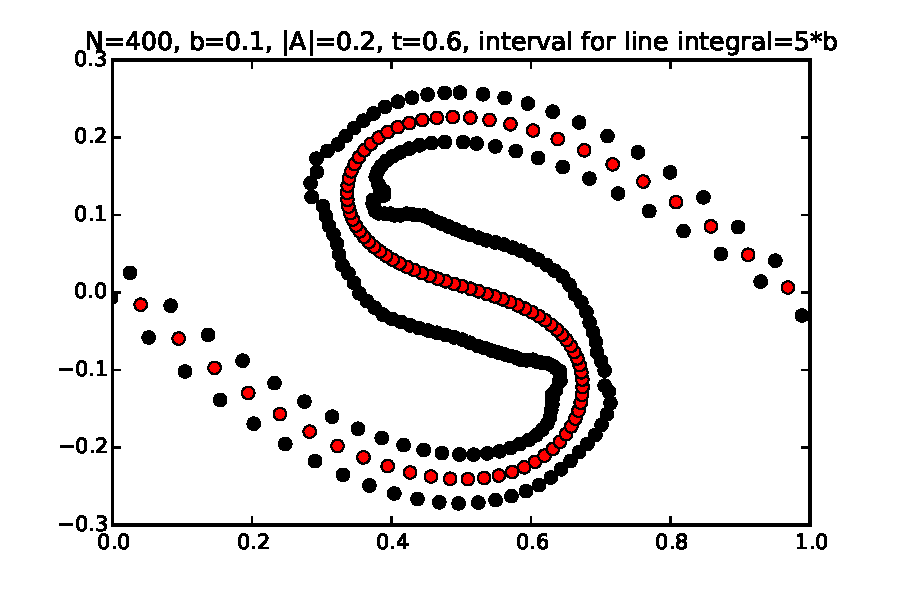
\includegraphics[width=3in,height=2in]{t06_B01.pdf}
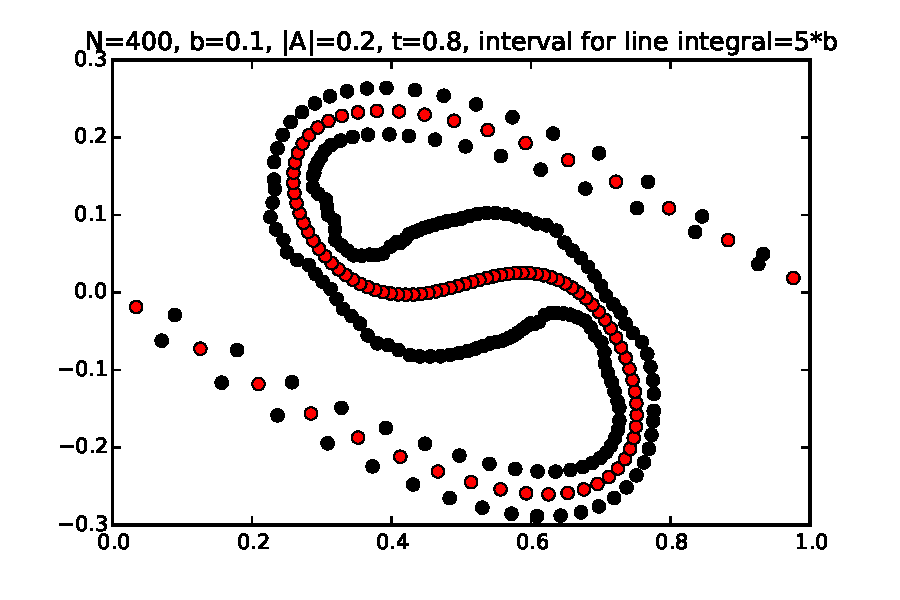
\includegraphics[width=3in,height=2in]{t08_B01.pdf}
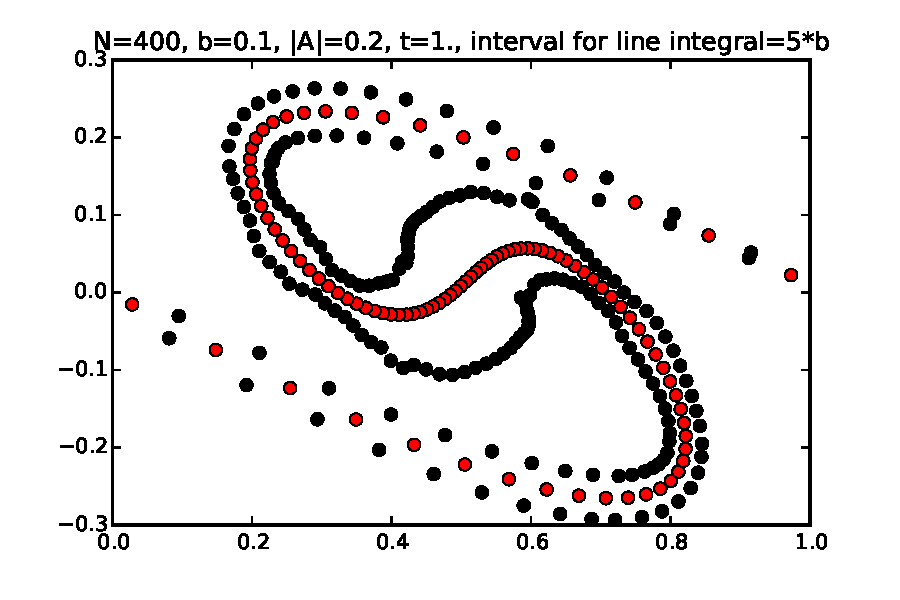
\includegraphics[width=3in,height=2in]{t10_B01.pdf}
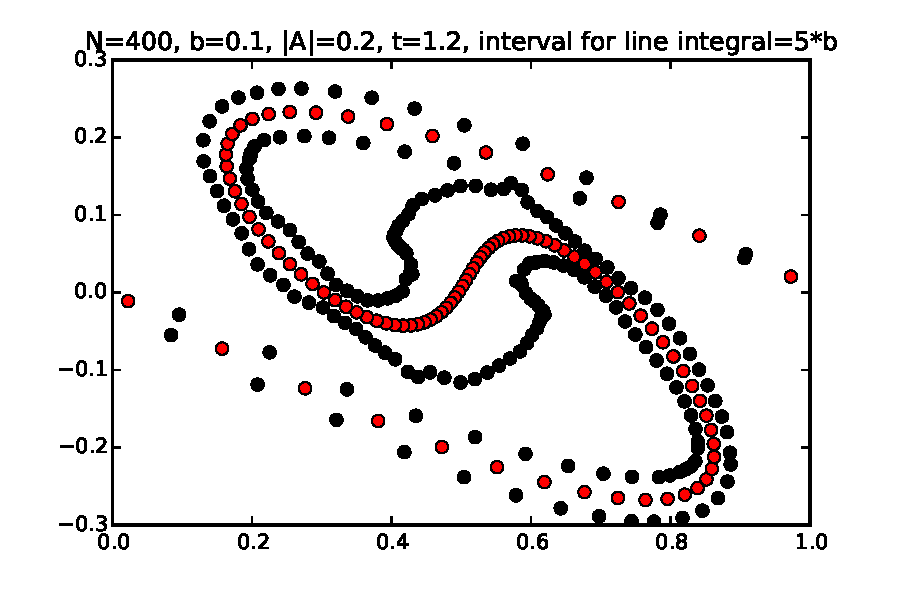
\includegraphics[width=3in,height=2in]{t12_B01.pdf}
\caption{$N=500 , \delta=0.05 ,  t=0.52$ }
\end{minipage}
\end{figure}



\end{document}
